\chapter{测试与评估}

本章将介绍基于Hyperledger Fabric的区块链云化框架的测试与评估工作。首先, 本章以典型案例的方式对原型工具进行功能性与非功能性测试;其次, 采用定性与定量方法论\cite{tashakkori1998mixed}结合五层成熟度模型以及与同类工具的对比对原型工具进行评估。

\section{原型工具测试}

\subsection{测试环境}

本文测试环境是在本地环境中进行, 测试环境采取Docker for Desktop搭建的单节点Kubernetes充当的集群环境, 具体配置如表\ref{computer}所示。

{\footnotesize
\begin{longtable}[h]{m{100pt} m{160pt}}
    \caption[配置详情]{配置详情} \label{computer} \\
        \toprule   
        \textbf{配置项目}&\textbf{配置详情}\\
        \hline
        CPU&4核\\
  
        内存&8G\\
    
        Swap&4G\\
        
        Docker for Desktop&Version 3.5.1\\
        
        Kubernetes&v1.21.2\\

        Fabric Ca&hyperledger/fabric-ca:1.4.9\\

        Fabric Peer&hyperledger/fabric-peer:amd64-2.3.0\\

        Fabric Orderer&hyperledger/fabric-orderer:amd64-2.3.0\\
        \bottomrule 
    \end{longtable} 
}

\subsection{测试流程}

本小节主要对原型工具进行功能性测试和非功能性测试。如图\ref{fabric_net}所示, 本节将以搭建最经典、简单的Fabric网络案例的方式进行完整的功能测试。测试重点针对于Ca、Peer、Orderer启动、创建通道、部署链码的全部过程, 验证Fabric网络启动及链码部署的正确性。最后, 本节 对安全性、数据可扩展性和监控体系进行测试。

\begin{figure}[h] %figure环境,h默认参数是可以浮动,不是固定在当前位置。如果要不浮动,你就可以使用大写float宏包的H参数,固定图片在当前位置,禁止浮动。
    \centering %使图片居中显示
    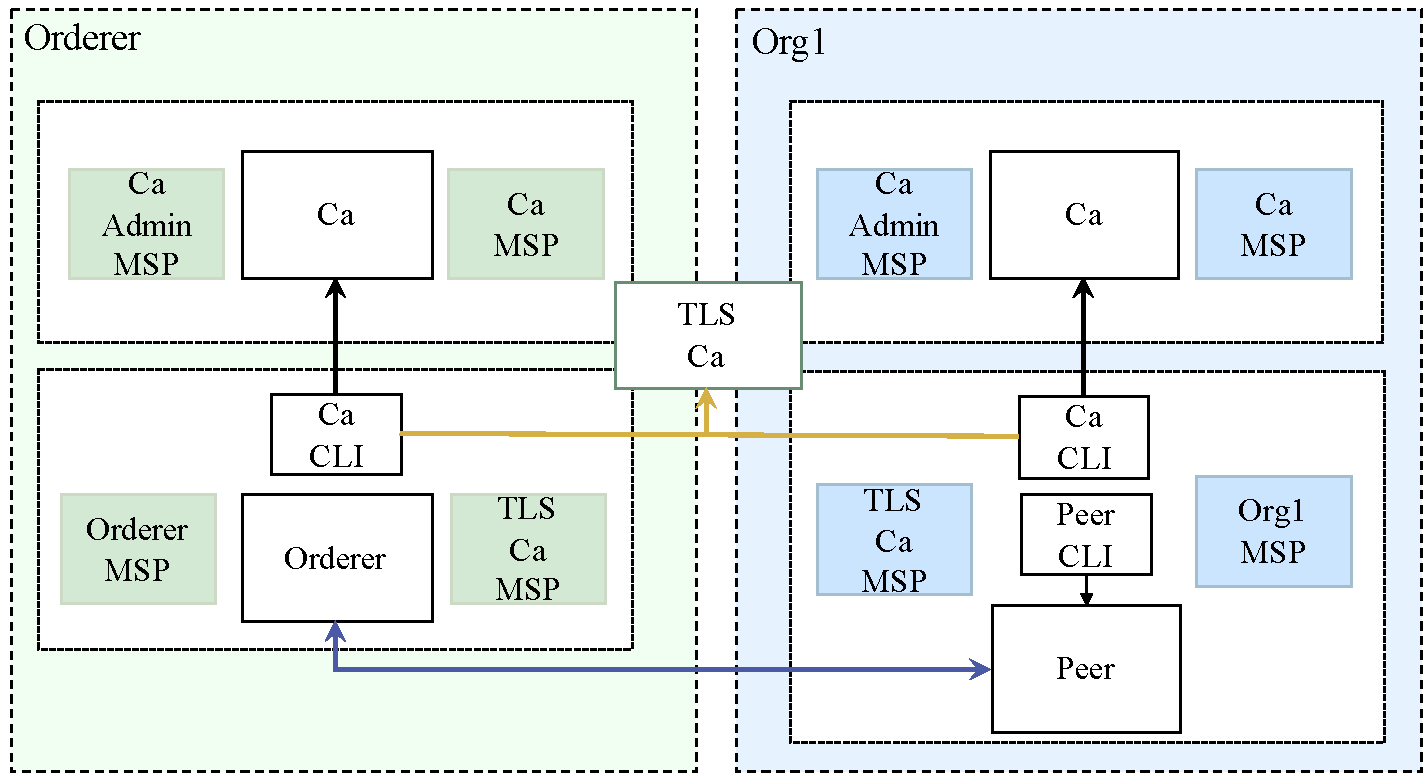
\includegraphics[width=0.9\textwidth]{FIGs/chapter5/fabric_net.pdf} %中括号中的参数是设置图片充满文档的大小,你也可以使用小数来缩小图片的尺寸。
    \caption{测试网络} %caption是用来给图片加上图题的
    \label{fabric_net} %这是添加标签,方便在文章中引用图片。
\end{figure}%figure环境


\textbf{步骤一:} 将原型工具部署入Kubernetes, 原型工具首先将内置的Fabric网络各节点的CRDs注入Kubernetes。如表\ref{org1_test}所示, Fabric网络管理员首先为org1创建了名为“org1-ca”的ca节点; 其次, 在org1中创建了名为“org1-peer0”的peer节点,并利用链外存储CouchDB作为账本存储单元。如图\ref{testcase1result}所示为测试结果, 原型工具可以为Fabric网络管理员创建Org1的Ca与Peer节点。

{\footnotesize
\begin{longtable}[h]{m{60pt}|m{280pt}}
    \caption[创建Org1测试用例]{Org1测试用例} \label{org1_test}\\
        \hline  
        ID&TC1\\
        \hline
        测试目标&创建含有一个Ca一个Peer的组织Org1\\
        \hline
        前置条件&原型工具已正常启动, Fabric网络各CRDs已经部署进Kubernetes\\
        \hline
        输入& (1)创建Ca节点:“kubectl-hlf ca create --name=org1-ca”;
        \newline (2)创建Peer节点:“kubectl-hlf peer create --name=org1-peer0 --mspid=Org1MSP --ca-name=org1-ca.default --db=CouchDB” \\

        \hline 
        预期输出& Org1内包含一个Ca节点以及一个Peer节点\\
        \hline
    \end{longtable} 
}


\begin{figure}[h] %figure环境,h默认参数是可以浮动,不是固定在当前位置。如果要不浮动,你就可以使用大写float宏包的H参数,固定图片在当前位置,禁止浮动。
    \centering %使图片居中显示
    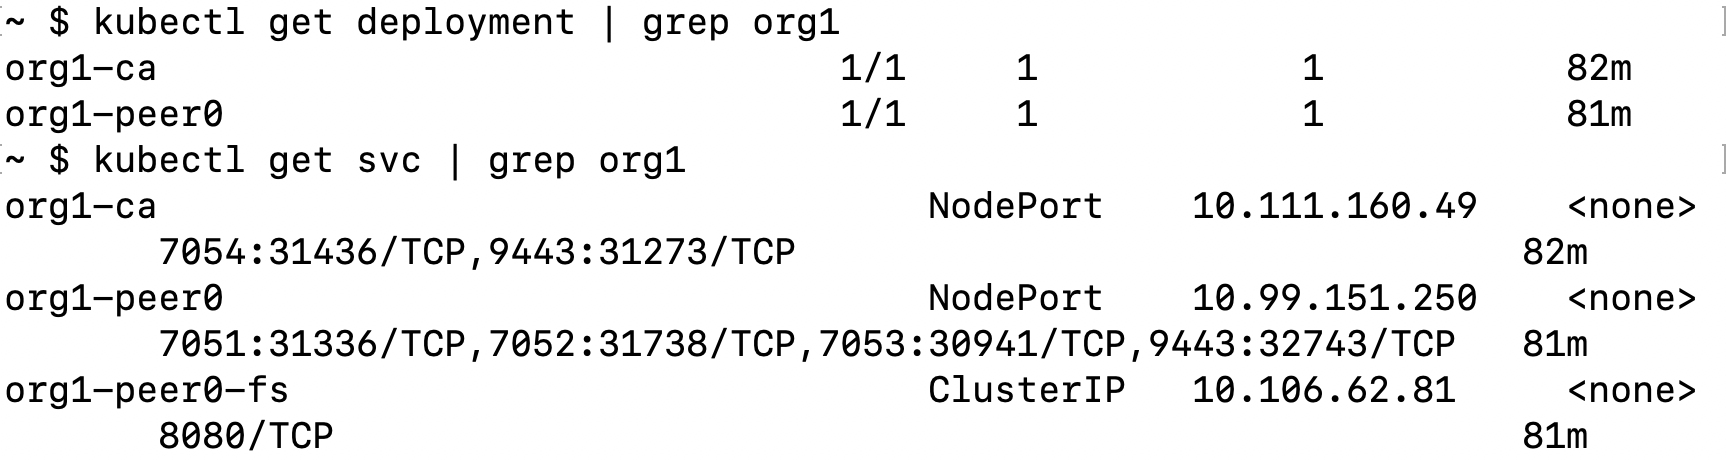
\includegraphics[width=0.9\textwidth]{FIGs/chapter5/peer.png} %中括号中的参数是设置图片充满文档的大小,你也可以使用小数来缩小图片的尺寸。
    \caption{创建Org1测试结果} %caption是用来给图片加上图题的
    \label{testcase1result} %这是添加标签,方便在文章中引用图片。
\end{figure}%figure环境

\newpage


\textbf{步骤二:} 如表\ref{orderer_test}所示, Fabric网络管理员需要首先为OrdererMSP创建名为“ord-ca”的ca节点; 其次, 在OrdererMSP中创建了名为“ord-node1”的peer节点。如图\ref{testcase2result}所示为测试结果, 原型工具可以为Fabric网络管理员创建Orderer的Ca与Orderer节点, 其中包含但不限于Deployment、Service、Pod、Secret等。

{\footnotesize
\begin{longtable}[h]{m{60pt}|m{280pt}}
    \caption[创建Orderer测试用例]{创建Orderer测试用例} \label{orderer_test}\\
        \hline  
        ID&TC1\\
        \hline
        测试目标&创建含有一个Ca一个Orderer的组织OrdererMSP\\
        \hline
        前置条件&原型工具已正常启动, Fabric网络各CRDs已经部署进Kubernetes\\
        \hline
        输入& (1)创建Ca节点:“kubectl-hlf ca create --name=ord-ca”;
        \newline (2)创建Orderer节点:“kubectl-hlf ordnode create --name=ord-node1 --mspid=OrdererMSP --ca-name=ord-ca.default” \\

        \hline 
        预期输出& OrdererMSP内包含一个Ca节点以及一个Orderer节点\\
        \hline
    \end{longtable} 
}

\begin{figure}[h] %figure环境,h默认参数是可以浮动,不是固定在当前位置。如果要不浮动,你就可以使用大写float宏包的H参数,固定图片在当前位置,禁止浮动。
    \centering %使图片居中显示
    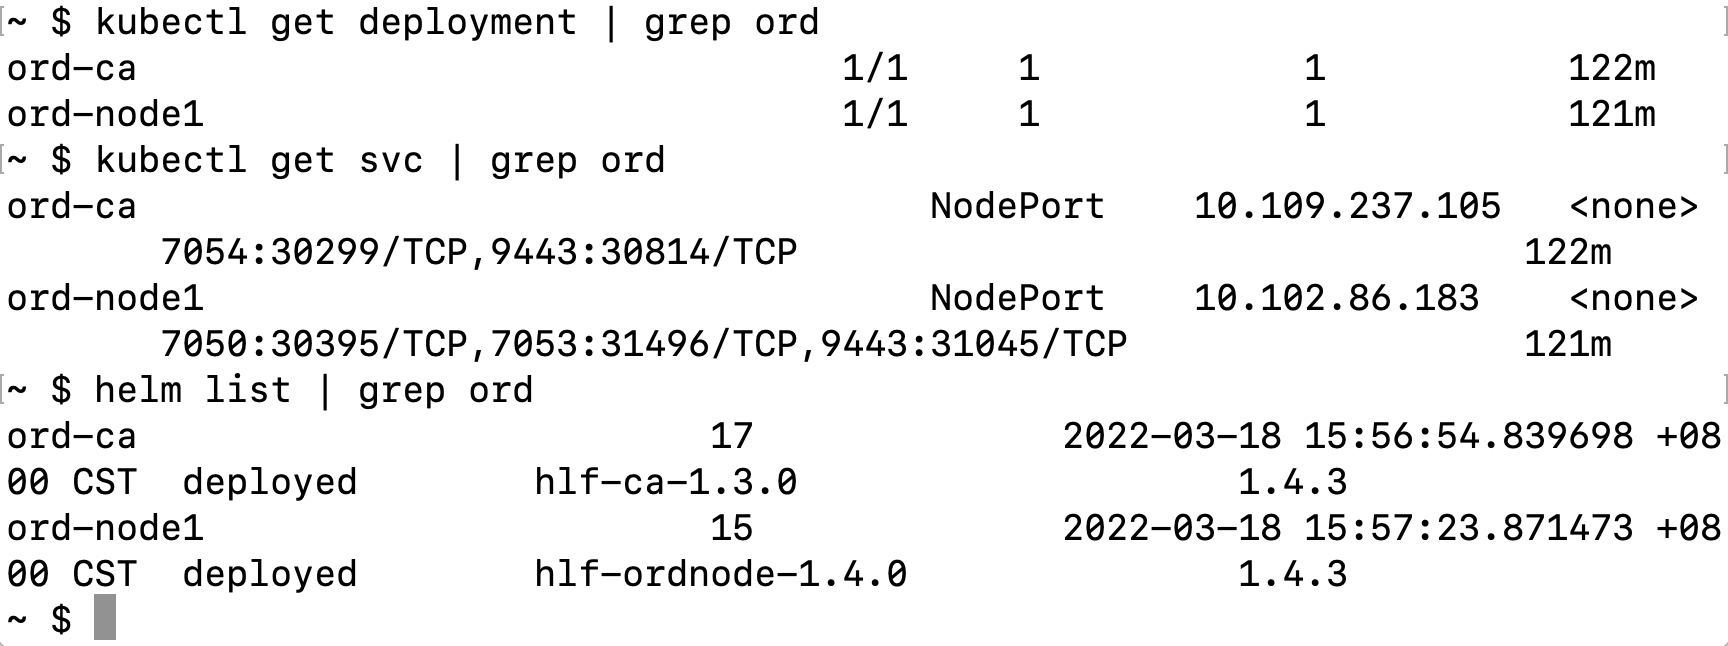
\includegraphics[width=0.9\textwidth]{FIGs/chapter5/orderer.png} %中括号中的参数是设置图片充满文档的大小,你也可以使用小数来缩小图片的尺寸。
    \caption{创建Orderer测试结果} %caption是用来给图片加上图题的
    \label{testcase2result} %这是添加标签,方便在文章中引用图片。
\end{figure}%figure环境

{\footnotesize
\begin{longtable}[h]{m{40pt}|m{300pt}}
    \caption[注册、登记用户测试用例]{注册、登记用户测试用例} \label{reg_enroll_test}\\
        \hline  
        ID&TC1\\
        \hline
        测试目标&分别为Orderer以及Org1注册、登记用户\\
        \hline
        前置条件&已经部署完成Orderer、以及Org1中的节点\\
        \hline
        输入& (1)导出Orderer信息:“kubectl-hlf inspect --output=orderer.yaml -o=OrdererMSP”
        \newline (2)注册用户:“kubectl-hlf ca register --name=ord-ca --user=ordereruser --secret=ordererpw --mspid=OrdererMSP”
        \newline (3)登记用户:“kubectl-hlf ca enroll --name=ord-ca --user=ordereruser --secret=ordererpw --mspid=OrdererMSP --output=orderer\_user.yaml”
        \newline (4)加入orderer.yaml:“kubectl-hlf utils adduser --userPath=orderer\_user.yaml --config=orderer.yaml --user=ordereruser --mspid=OrdererMSP”\\

        \hline 
        预期输出& (1)包含ordereruser用户密钥证书信息的orderer\_user.yaml
        \newline (2)包含OrdererMSP所有信息的orderer.yaml\\
        \hline
    \end{longtable} 
}

\textbf{步骤三:} 如表\ref{reg_enroll_test}所示, Fabric网络管理员需要为OrdererMSP以及Org1注册并登记若干用户, 并将用户的证书密钥信息导到yaml文件中。表中仅展示在Orderer中注册用户, Org1中步骤相似(Org1信息输出为org1.yaml)。测试结果表明, 可以成功将用户及OrdererMSP信息导出。


\textbf{步骤四:} 如表\ref{channel_test}所示, Fabric开发人员需要在新创建的Fabric网络上创建通道, 并初始化该通道内的创世区块。当通道被创建完成之后, 需要将在该通道内进行交易的的Orderer、Peer加入该通道。最后, Fabric开发人员可以指定锚节点并查看通道的高度。如图\ref{channel_test_result}所示为测试结果, 展示了新创建的通道的高度。

{\footnotesize
\begin{longtable}[h]{m{60pt}|m{280pt}}
    \caption[创建通道测试用例]{创建通道测试用例} \label{channel_test}\\
        \hline  
        ID&TC1\\
        \hline
        测试目标&创建通道并将创世节点、org1-peer0加入通道\\
        \hline
        前置条件&已经查创建组织并生成相应用户\\
        \hline
        输入& (1)创建通道:“kubectl-hlf channel generate --output=demo.block --organizations Org1MSP --ordererOrganizations OrdererMSP”;
        \newline (2)将Orderer加入通道:“kubectl-hlf ordnode join --name=ord-node1”
        \newline (3)将Peer加入通道:“kubectl-hlf channel join --name=testchannel --user=peeruser --config=org1.yaml -p=org1-peer0”
        \newline (4)检视通道:“kubectl-hlf channel inspect --name=testchannel --user=peeruser --config=org1.yaml -p=org1-peer0 > testchannel.json”
        \newline (5)指定锚节点:“kubectl-hlf channel addanchorpeer --name=testchannel --user=peeruser --config=org1.yaml -p=org1-peer0”
        \newline (6)查看通道高度:“kubectl-hlf channel top --name=testchannel --config=org1.yaml --user=admin -p=org1-peer0”\\

        \hline 
        预期输出& (1)成功创建通道并将创世节点、org1-peer0加入通道
        \newline (2)成功获取通道信息testchannel.json
        \newline (3)成功展示通道高度\\
        \hline
    \end{longtable} 
}

\begin{figure}[h] %figure环境,h默认参数是可以浮动,不是固定在当前位置。如果要不浮动,你就可以使用大写float宏包的H参数,固定图片在当前位置,禁止浮动。
    \centering %使图片居中显示
    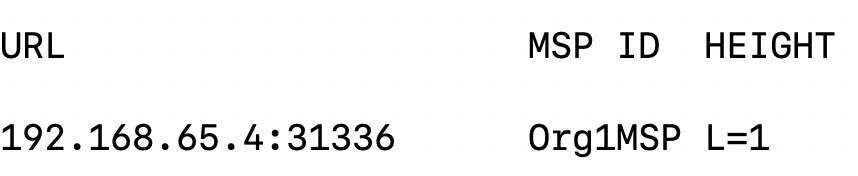
\includegraphics[width=0.55\textwidth]{FIGs/chapter5/channel.png} %中括号中的参数是设置图片充满文档的大小,你也可以使用小数来缩小图片的尺寸。
    \caption{查看通道高度测试结果} %caption是用来给图片加上图题的
    \label{channel_test_result} %这是添加标签,方便在文章中引用图片。
\end{figure}%figure环境

\textbf{步骤五:} 如表\ref{chaincode_test}所示, 为测试通道内所有的参与节点按照链码的合同规则执行, Fabric开发人员需要在新创建的通道内安装官方提供的asset\footnotemark[1]\footnotetext[1]{\href{https://github.com/hyperledger/fabric-samples/blob/main/asset-transfer-basic/chaincode-go/chaincode/smartcontract.go}{asset链码 github地址}}链码, 安装完链码之后, 需要对其进行审批、提交。最后, Fabric开发人员可以调用链码接口对其进行初始化、查询等一系列操作。如图\ref{chaincode_test_result}所示为测试结果, 展示了查询链码之后的结果。

{\footnotesize
\begin{longtable}[h]{m{60pt}|m{280pt}}
    \caption[链码相关测试用例]{链码相关测试用例} \label{chaincode_test}\\
        \hline  
        ID&TC1\\
        \hline
        测试目标&安装、审批、提交、调用、查询链码\\
        \hline
        前置条件&已经成功启动通道\\
        \hline
        输入& (1)安装链码:“kubectl-hlf chaincode install --path=asset --user=peeruser --config=org1.yaml --language=golang --label=asset --peer=org1-peer0;
        \newline (2)查询链码:“kubectl-hlf chaincode queryinstalled --user=peeruser --config=org1.yaml --peer=org1-peer0”;
        \newline (3)审批链码:“kubectl-hlf chaincode approveformyorg --user=peeruser --config=org1.yaml --peer=org1-peer0 --package-id=PACKAGEID --name=asset --policy=POLICY --channel=testchannel”;
        \newline (4)提交链码:“kubectl-hlf chaincode commit --config=org1.yaml --peer=org1-peer0 --name=asset --policy=\$POLICY --channel=testchannel”
        \newline (5)调用链码:“kubectl-hlf chaincode invoke --config=org1.yaml --peer=org1-peer0 --chaincode=asset --channel=testchannel --function=FUNCTION”
        \newline (6)查询链码:“kubectl-hlf chaincode query --config=org1.yaml --peer=org1-peer0 --chaincode=asset --channel=testchannel --function=\$FUNCTION”\\
        \hline 
        预期输出& 成功安装、查询、审批、提交、调用、查询链码\\
        \hline
    \end{longtable} 
}

\begin{figure}[h] %figure环境,h默认参数是可以浮动,不是固定在当前位置。如果要不浮动,你就可以使用大写float宏包的H参数,固定图片在当前位置,禁止浮动。
    \centering %使图片居中显示
    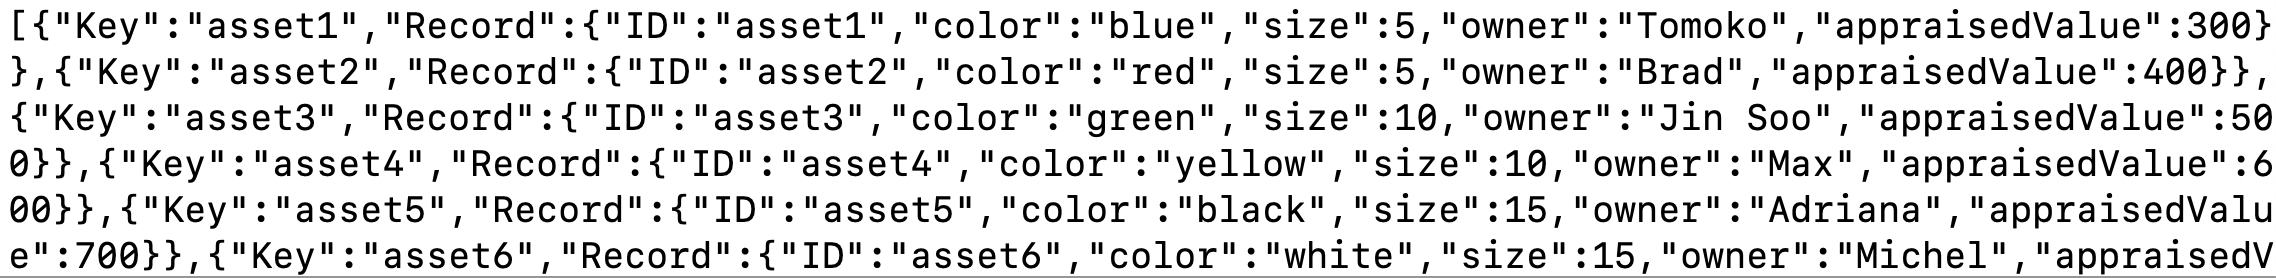
\includegraphics[width=1.0\textwidth]{FIGs/chapter5/chaincode.png} %中括号中的参数是设置图片充满文档的大小,你也可以使用小数来缩小图片的尺寸。
    \caption{查询链码} %caption是用来给图片加上图题的
    \label{chaincode_test_result} %这是添加标签,方便在文章中引用图片。
\end{figure}%figure环境


\begin{figure}[h] %figure环境,h默认参数是可以浮动,不是固定在当前位置。如果要不浮动,你就可以使用大写float宏包的H参数,固定图片在当前位置,禁止浮动。
    \centering %使图片居中显示
    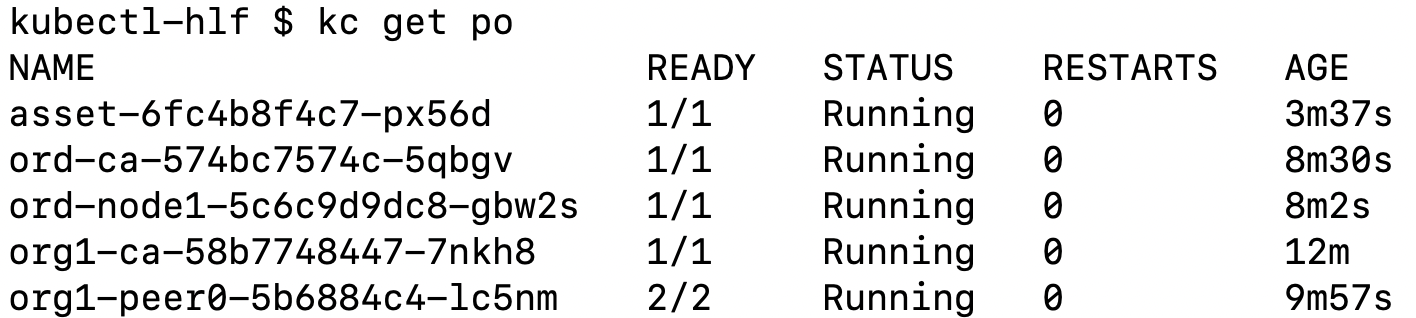
\includegraphics[width=1.0\textwidth]{FIGs/chapter5/fabric_result.png} %中括号中的参数是设置图片充满文档的大小,你也可以使用小数来缩小图片的尺寸。
    \caption{网络节点状态} %caption是用来给图片加上图题的
    \label{fabric_result} %这是添加标签,方便在文章中引用图片。
\end{figure}%figure环境

经过上述步骤1-5, 最终的网络节点状态如图\ref{fabric_result}所示, 本文搭建了一个单Orderer以及单Org、单Peer的简单的Fabric网络, 并分别Orderer、以及Peer搭配Ca证书认证。在搭建了基本的网络之后, 分别为Orderer、Peer注册并登记用户, 最后在组织Org中搭建了一个通道并成功安装调用链码。测试结果可知, 本文的原型工具能够正常成功搭建Fabric网络及部署链码。

本文接下来对原型工具的非功能性需求进行测试, 查看原型工具是否满足第\ref{section: requirement}节所提到的易用性、可扩展性、安全性等非功能性需求。

易用性, 本文邀请了5位熟悉Hyperledger Fabric基本概念及网络搭建流程的开发人员对本文的原型工具进行易用性测试。为了排除网络的影响,
本文提前下载好原型工具搭建Fabric网络所需要的Docker镜像。在介绍了本工具的基本原理以及命令行的基本使用方法后, 5位测试的开发人员分别独立自行搭建不同规格的Fabric网络, 最终5为测试的开发人员都能够在30分钟内学习并掌握原型工具的使用方法。

为测试本工具的可靠性, 本文在使用原型工具搭建Fabric网络过程中有意输入错误的命令行参数, 输入不正确的密钥文件等, 原型工具都能在1s内给出参数的异常情况; 同时, 在搭建完Fabric网络之后, 原型工具在两周内仅崩溃1次, 且能在5分钟内进行恢复。

可迁移性

可扩展性

安全性



\section{原型工具评估}

\subsection{五层成熟度模型}

如图所示\ref{maturity}, Kubernetes operator拥有5个成熟度级别的定义\cite{duan2021case}, 其通过定性的方式分析某个operator应用是否达到了某个级别, 这5个成熟度级别定义如下:

\begin{itemize}[itemindent=2em]
    \item 第一级: Basic Intall, 该级是operator成熟度模型中最基本的级别。在该级中, 用户能够使用CRD对目标程序进行配置和安装;

    \item 第二级: Seamless Upgrades, 在该级别上的operator能够不丢失数据的升级所管理的工作负载;

    \item 第三级: Full Lifecycle, 是否能达到该级别取决于operator是否具备生命周期管理和的数据备份、恢复能力。在该级别上的operator能够备份数据, 并在发生任何数据灾难时从备份数据中恢复数据。

    \item 第四级: Deep Insights, operator提供监控和报警等功能。在该级别, operator能够包含所有组件的运行状况指标, 并根据指标配备报警功能;

    \item 第五级: Auto Pilot, 最终级别拥有许多高级功能, 如自动伸缩。operator可以通过收集到的指标来扩展工作负载。

\end{itemize}

\begin{figure}[h] %figure环境,h默认参数是可以浮动,不是固定在当前位置。如果要不浮动,你就可以使用大写float宏包的H参数,固定图片在当前位置,禁止浮动。
    \centering %使图片居中显示
    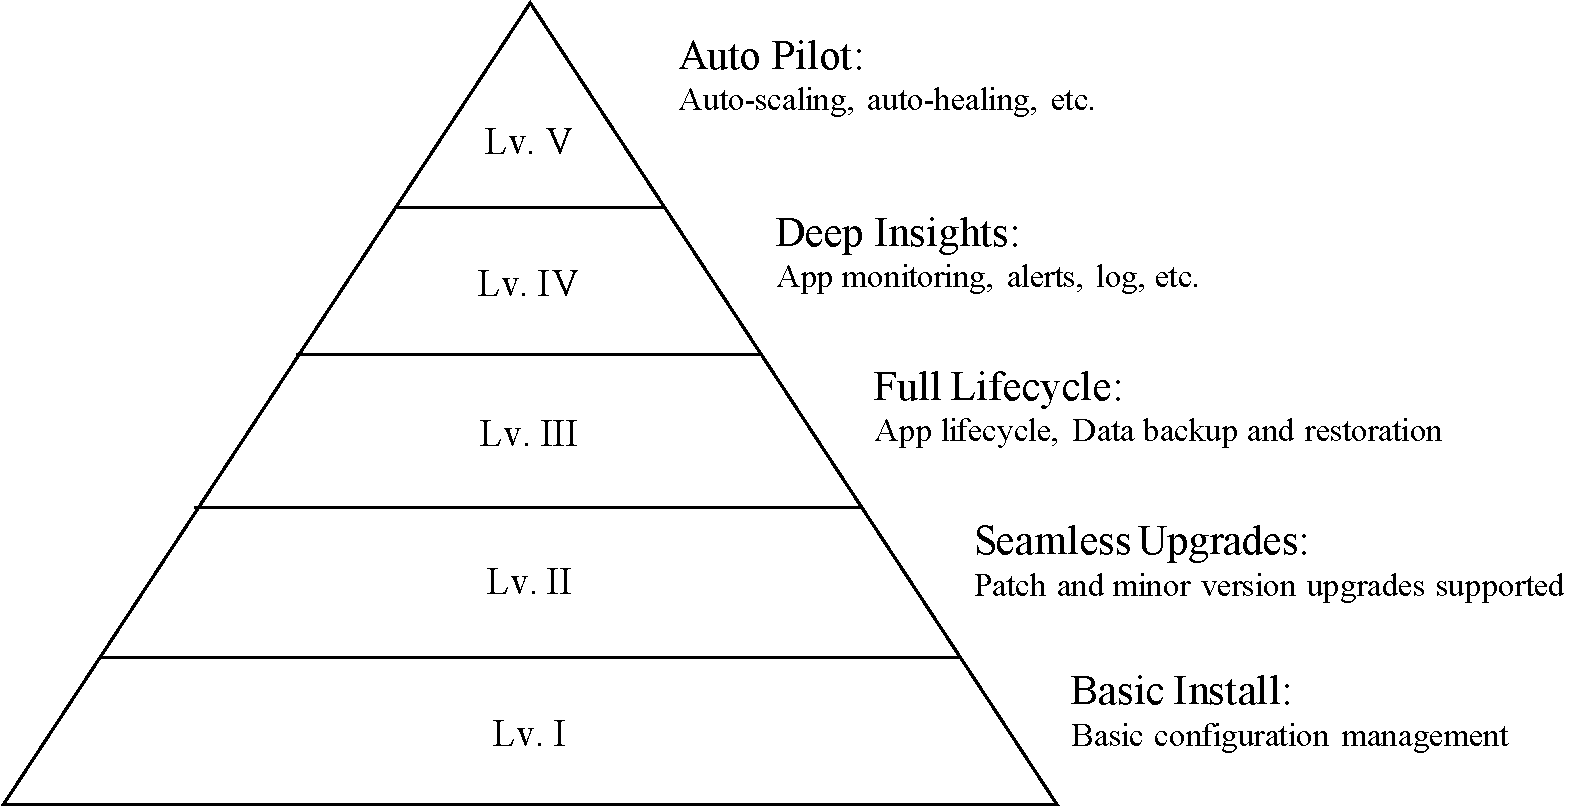
\includegraphics[width=0.85\textwidth]{FIGs/chapter5/maturity.pdf} %中括号中的参数是设置图片充满文档的大小,你也可以使用小数来缩小图片的尺寸。
    \caption{成熟度模型} %caption是用来给图片加上图题的
    \label{maturity} %这是添加标签,方便在文章中引用图片。
\end{figure}%figure环境

\textbf{Basic Install}

借助于原型工具, 能够通过命令行方式一键启停Fabric网络中任意节点, 而且不需要进行复杂的证书管理。一旦原型工具被部署在Kubernetes网络中, 原型工具就可以对CRs以及helm进行管理, Fabric网络管理人员可以借助命令行参数的方式进行创建、更新CRs以此来创建特定规格的Fabric网络。 一旦CRs进行更新, 原型工具就会将当前状态调整为与指定状态一致。

\textbf{Seamless Upgrades}

在原型工具中, Fabric网络管理员可以通过修改CRs的内容对包括Fabric网络节点镜像、端口、host、版本等进行无缝修改。此外, 由于原型工具依赖于链外存储的CouchDB, 以及外部的Prometheus监控体系, 这两者的升级并不会对原型工具产生严重的负面影响。 

\textbf{Full Lifecycle}

虽然原型工具能够在mangager中对结合helm对Fabric网络进行全生命周期管理, 但目前原型工具目前仍缺少数据备份和恢复的能力。要达到这一能力需要在CRs中指定远程备份的数据存储平台, 并在CRs中指定数据备份的凭证以及远程备份的链接。同时, 原型工具在一定的时间周期内将数据备份的到远程的数据存储平台上。

\textbf{Deep Insights}

原型工具利用Prometheus监控体系实现监控与报警的功能, 与此同时, 除了让Prometheus抓取pod的基本指标外, CRD中还设定了PodMonitor、ServiceMonitor、CouchDBExporter接口, 可以让Prometheus更全面的抓取Fabric网络的监控指标。Fabric网络管理员可以通过Grafna可视化图表查看整体Fabric网络运行状态, 并且能够根据监控指标创建自定义的告警规则。

\textbf{Auto Pilot}

在Kubernetes中存在两种自动伸缩的插件, 即HPA、VPA。当负载超过一定的阈值时, 就会对其进行伸缩或配置更多的资源。然而在Fabric网络中, 每个peer都有记录全部账本的职责, 并且只需要超过51\%的peer节点保持一致即可, 所以针对于peer并不需要根据监控进行自我伸缩的能力。在数据存储方面, 随着账本的膨胀, 原型工具可以针对链外存储进行扩容。

综上, 本文原型工具利用operator管理Fabric网络能够完美的具备第一级、第二级在第三级上能够支持全生命周期管理但是对于数据的备份能力依旧是存在欠缺, 借助原型工具实现了第四级的监控, 对于自动伸缩方面仅支持数据层面的扩展, 所以本文原型工具基本满足5层成熟度模型的功能。



\section{本章小结}

本章介绍了对战术建模支持方法及工具的测试和案例研究。
首先设计测试用例对建模支持工具的“可视化建模”、“建模约束校验”、“模型存储”以及“生成项目”
功能进行了测试,还通过在具体案例中执行建模的五个步骤对建模支持方法及工具进行了验证。
